\documentclass[submit,techrep,noauthor]{ipsj}
\usepackage[dvipdfmx]{graphicx}
\usepackage{latexsym}
\usepackage{algorithm}
\usepackage{algorithmic}
\usepackage{amsmath}
\usepackage{url}

\begin{document}

\title{Token log確率を用いた\\Verilogコード生成候補の問題依存的不確実性誘導テスト}

\affiliate{NU}{名古屋大学\\
Nagoya University}

\author{椋木大地}{Daichi Mukunoki}{NU}
\author{林俊一郎}{Shunichiro Hayashi}{NU}
\author{星野哲也}{Tetsuya Hoshino}{NU}
\author{片桐孝洋}{Takahiro Katagiri}{NU}

\begin{abstract}
LLMによるVerilogコード生成では，複数の候補を生成しても，最終的にはコンパイル，elaboration，simulationを通したvalidationが必要である．候補数を増やすほど正しい実装を含む可能性は高まるが，その分だけvalidation costも増える．このcostを下げる自然な方法は，LLMが出力するtoken-level log確率を用いて有望な候補を先に試すcandidate rankingである．しかし，VerilogEval code-complete-iccad2023 156問・100 trials・$k=10$候補の評価では，平均log確率，25パーセンタイル，最小log確率によるcandidate rankingは，コンパイル失敗候補を後回しにする一方で，コンパイル通過後のsemantic correctnessを十分に識別できなかった．本研究ではこの結果を踏まえ，token log確率を候補全体の正解度スコアとしてではなく，どこを重点的にvalidationすべきかを示す局所的不確実性信号として用いる．提案手法Hybrid Uncertainty-Guided Testing（Hybrid-UGT）は，低log確率token周辺のspanから信号名，bit範囲，演算子，case/state，reset/clockを抽出し，参照実装をoracleとする固定テンプレートtestbench向けのdirected validation inputを生成する．compile-pass official-fail候補のうち，生成token数$\le512$の全件である31,842候補に対するオフラインfailure detection評価を行った．本評価における主要な観察は，Hybrid-UGTがdetection budgetの小さい領域（det@1）でRandomを明確に上回り，budgetを増やすほどRandomが追いつくという性能曲線である．全体でHybrid-UGTのdet@1は0.524でRandomの0.496を$+0.028$上回り（候補単位paired bootstrap 95\% CI $[+0.022, +0.034]$），counter系（n=2,375）で$+0.146$ det@1（CI $[+0.126, +0.166]$），posedge clock系（n=13,867）で$+0.069$，FSM/state遷移系（n=3,889）で$+0.059$，shift/rotate系（n=3,139）でも$+0.053$ det@1の優位を示した．一方で，det@16ではHybrid-UGT 0.841，Random 0.845と同等に収束し（$\Delta = -0.005$, CI $[-0.007, -0.002]$），shift/rotate系ではdet@16で$-0.061$（CI $[-0.078, -0.044]$）と顕著に劣後する．Hybrid-UGTは「少数validation vectorで明らかな失敗候補をfail-fast棄却する」per-request screeningの用途に整合する性能特性を示すが，16ベクトルまで全予算を消化すれば，両手法の累積検出率はほぼ等しい．本評価はper-request候補screeningにおけるuniform random比較であり，産業的に用いられるconstrained random verificationを代替するものではない．
\end{abstract}

\maketitle

\section{はじめに}

LLMのコード生成能力は，Codex\cite{chen2021codex}やAlphaCode\cite{li2022alphacode}以降，大きく向上している．しかし，実用的なコード生成では，LLMの出力をそのまま採用するのではなく，コンパイル，test，性能評価などで候補を選択する必要がある．VerilogのようなHDLコード生成では，このvalidationはさらに重要である．生成候補は構文解析，elaboration，testbenchとの結合，simulationを通して検証され，参照実装や仕様と出力が一致して初めて採用できる．

複数候補生成は，少なくとも1つの正しい候補を得るための有効な方法である．一方で，候補数を増やすほどvalidation costも増える．特にHDLでは，候補ごとにコンパイル，elaboration，simulationを実行する必要があり，より重いfull validationや回帰testに進む前に，明らかに失敗する候補を早く除外できることが望ましい．

この目的に対して，LLMが各tokenに付与するlog確率は一見有望である．高log確率のtoken列はモデルにとって自然な実装に見えるため，平均log確率などで候補を並べ替えれば，正しい候補を早く見つけられるように思える．しかし，Verilogでは，高log確率で自然に見えるコードであっても，仕様解釈，境界条件，状態遷移，bit幅，part-selectを誤ることがある．つまり，token log確率を候補全体の正解確率として扱うcandidate rankingには限界がある．

本研究の発想は，log確率を候補全体のscoreとして使うのではなく，局所的なvalidation focusとして使うことである．低log確率tokenは，モデルがその位置で迷った箇所を示す可能性がある．Verilogでは，信号名，bit範囲，演算子，\texttt{case}文，\texttt{posedge}，\texttt{reset}などがコード上に明示的に現れるため，低確信度spanをinput stimulusやclock sequenceに変換しやすい．したがって，低確信度spanは「どの入力信号やbit範囲を重点的に動かすべきか」を決める手掛かりになり得る．

本稿の提案手法はHybrid Uncertainty-Guided Testing（Hybrid-UGT）である．Hybrid-UGTは，まず少数のrandom smoke inputを実行し，容易に露呈する誤りを検出する．次に，低log確率token周辺のspanを解析し，そのspanに現れる入力信号，bit範囲，演算子，状態遷移，reset/clockに基づいてdirected validation inputを生成する．生成したinput sequenceは固定テンプレートのtestbenchに埋め込まれ，候補実装\texttt{TopModule}と参照実装\texttt{RefModule}を同じ入力で駆動して出力不一致を検出する．このsmall validationは正しさを証明するものではなく，重いfull validationの前に失敗候補を早く発見するscreeningとして位置づける．

本研究の貢献は以下の3点である．
\begin{itemize}
\item \textbf{VerilogEvalにおけるcandidate rankingの限界分析}: 候補全体の平均log確率，25パーセンタイル，最小log確率によるcandidate rankingを評価し，token log確率はコンパイル失敗候補の後回しには有効だが，コンパイル通過後のsemantic correctness識別には限定的であることを示す．
\item \textbf{Hybrid-UGTの提案とfocus型directed inputの再現可能な実装}: 低log確率tokenを局所的不確実性spanとして扱い，span内のVerilog構文要素から小規模directed validation inputを生成する手法を提案する．本稿では入力ベクトル生成器，固定テンプレートtestbench，iverilog/vvpシミュレータ連携，5手法（Random，Generic，Category-UGT，Span-UGT，Hybrid-UGT）の評価器を実装し，全モジュールをgit管理下で再現可能な形で公開する．
\item \textbf{Detection-budget依存性の特定}: compile-pass official-fail候補のうち生成token数$\le 512$の全件31,842候補に対する評価では，Hybrid-UGTがRandomを上回るのは小さい$B$におけるdet@$B$である．全体でdet@1は$0.524$と$0.496$で$+0.028$，counter系（n=2,375）で$+0.145$ det@1，posedge clock系（n=13,867）で$+0.068$ det@1，FSM/state遷移系（n=3,889）で$+0.058$ det@1の優位を示す．一方，$B=16$まで予算を増やすと両手法は$0.845$近傍でほぼ等値（$\Delta = -0.004$）に収束する．Hybrid-UGTは「少数vectorで明らかなfailを早く落とす」用途に有用で，full budget評価では優位性が出ない．
\end{itemize}

以下，第2章で関連研究，第3章で予備知識，第4章で提案手法，第5章で実験設定，第6章で結果，第7章で考察，第8章で制約，第9章で結論を述べる．

\section{関連研究}

\subsection{コード生成と候補選択}

Codex\cite{chen2021codex}やAlphaCode\cite{li2022alphacode}は，複数候補を生成し，テスト実行やクラスタリングにより候補を選択することでコード生成性能を高めた．Self-Consistency\cite{wang2023selfconsistency}は，複数の推論経路をサンプリングし，一貫した解を選ぶ枠組みを示した．CodeT\cite{chen2022codet}は生成テストを用いて候補を評価し，CodeRL\cite{le2022coderl}はテスト結果を報酬として利用する．これらはテストや実行フィードバックを利用して候補を選択する点で本研究と関連する．本稿は，テスト前に得られるtoken log確率を，追加validation input generationの焦点決定に用いる点が異なる．

\subsection{不確実性を用いたLLM出力制御}

Semantic Entropy\cite{semantic_entropy2024}は，意味的に同じ出力をクラスタリングし，意味空間でのエントロピーを計算することで幻覚検出を改善した．Code Semantic Entropy\cite{code_semantic_entropy2026}は，コードの振る舞いの多様性に基づいて問題レベルの不確実性を測定する．Token-level不確実性に関しては，TokUR\cite{tokur2025}やtoken-level uncertainty-aware objective\cite{token_uq_training2025}が，token単位の信頼度評価や訓練目的への応用を検討している．

コード生成への応用として，USCD\cite{uscd2024}はtoken-level不確実性を用いた選択的対比デコーディングを提案し，Sharmaら\cite{assess_correctness2025}はsymbolic executionで意味的等価性をクラスタリングすることでコード生成候補の正しさを不確実性で評価した．Xuら\cite{riscoset2026}は，token-level negative log probabilityをAST node単位の信頼度として用い，Learn Then Testフレームワークで「正解プログラムを高確率で含むpartial programの集合」を構築するRisCoSetを提案した．本研究は，これらの「候補全体の正しさ予測」や「prediction setの構築」とは異なり，低確信度spanを生成後validation inputの焦点として用いる点で異なる．

\subsection{適応的デコーディングと反復的改善}

AdaDec\cite{adadec2025}は，生成中のtoken-level不確実性を用いてpause-then-rerankを行う適応的デコーディング手法である．AdapT\cite{adapt2023}やEDT\cite{edt2024}は，tokenごとまたはステップごとに温度を適応的に調整する．Self-Refine\cite{madaan2023selfrefine}は，LLM自身による反復的フィードバックと改善を提案した．これらは生成過程や再生成過程を制御する手法である．本稿では，生成済み候補を固定したまま，低確信度spanを用いて追加validation inputを生成する後処理を扱う．

\subsection{Verilogコード生成評価}

VerilogEval\cite{liu2023verilogeval}は，HDLBits由来のVerilogコード生成評価ベンチマークであり，問題文，\texttt{TopModule}のインタフェース，参照実装，testbenchを提供する．生成候補は参照実装とのsimulation出力比較により評価される．Verilogは，bit幅，信号名，状態遷移，clock/resetなどの構造が明示的であり，低確信度spanを具体的なinput stimulusへ変換しやすい．この性質を利用する点が，本研究のVerilog専用ストーリーの中心である．

\section{予備知識}

\subsection{VerilogEval code-completeタスク}

本稿ではVerilogEval code-complete-iccad2023を用いる．このタスクでは，自然言語の仕様と\texttt{TopModule}のポート定義が与えられ，モデルはモジュール本体を補完する．各問題には参照実装\texttt{RefModule}と公式testbenchが含まれる．候補\texttt{TopModule}は，Icarus Verilogにより公式testbenchおよび参照実装とともにコンパイルされ，simulation出力が参照実装と一致すれば成功と判定される．

VerilogEvalの問題は公式カテゴリを持たないため，本稿では公開されている問題名，仕様，参照実装の構文特徴に基づいて，simple logic，procedural combinational，arithmetic datapath，sequential datapath，FSM/controlの5種類に分類する．この5種類分類は問題単位の排他的分類であり，主に評価対象集合の構成と全体サマリの集計軸として用いる．これに加えて§\ref{sec:problem_dependence}では，個々の候補コードが含む構文構造（counter，shift/rotate，case，always\_comb等）に基づく多ラベル分類を別途定義し，問題依存性の細かい分析に用いる．いずれの分類も提案手法の実行時入力としては用いない．

\subsection{token log確率}

自己回帰LLMは，それまでのtoken列$t_1,\ldots,t_{i-1}$に基づき，次token$t_i$の条件付き確率$P(t_i|t_1,\ldots,t_{i-1})$を計算する．生成時に返されるlog確率を
\begin{equation}
\ell_i = \log P(t_i|t_1,\ldots,t_{i-1})
\end{equation}
とする．候補コード$c$の平均log確率は
\begin{equation}
\mathrm{Mean}(c)=\frac{1}{N}\sum_{i=1}^{N}\ell_i
\end{equation}
であり，候補全体のtoken列の自然さを表す．本稿では，log確率列の25パーセンタイルを
\begin{equation}
\mathrm{Tail}(c)=Q_{0.25}(\{\ell_i\}_{i=1}^{N})
\end{equation}
と定義し，候補中の最小log確率を\(\mathrm{MinLogP}(c)=\min_i \ell_i\)と呼ぶ．

これらの集約スコアはcandidate rankingに使えるが，平均値，分位点，最小値はいずれも候補全体を1つの数値に潰す．Hybrid-UGTでは，集約スコアではなく，低log確率tokenの位置そのものを用いる．

\subsection{validation inputとtestbench template}

本稿で生成する対象は，LLMが書いたtestbenchコードではなく，候補を検査するvalidation input vector列である．validation input vector列は，候補実装と参照実装を同じ入力で駆動する固定テンプレートのtestbenchに埋め込む．このtestbenchはVerilogEvalの公式testbenchを置き換えるものではなく，参照実装または等価なoracleが利用できる場面で，出力不一致を早期に検出するsmall screening validationコードである．概念的には以下の形を取る．

\begin{quote}
\small
\texttt{RefModule ref\_i (...);}\\
\texttt{TopModule dut\_i (...);}\\
\texttt{生成したvalidation input vectorを順に与える;}\\
\texttt{各入力でref\_iとdut\_iの出力を比較する;}
\end{quote}

組合せ回路では，各validation input vectorは1つの入力割当を表す．順序回路では，固定テンプレートがclockを駆動し，各validation input vectorを1サイクル分の入力割当として順に与える．clockはテンプレート側で制御するため，RandomやHybrid-UGTが値をサンプルする入力には含めない．reset信号は，信号名やspan中の記述から推定できる場合にdirected inputの対象とし，推定できない場合は通常入力と同じ固定規則で扱う．

このテンプレートtestbenchで不一致が出た候補は失敗候補として棄却できる．一方，不一致が出ないことは正しさの証明ではないため，最終的には公式testbenchやより重いfull validationが必要である．

\section{提案手法}\label{sec:method}

\subsection{問題設定}

1つの問題$p$に対して，LLMはVerilog候補$c$を生成し，生成token列とlog確率列を返す．本稿では，候補コードそのものを修復したり再生成したりせず，候補$c$を検証するための小規模validation input vector列$V=\{v_1,\ldots,v_B\}$を生成する．評価では，参照実装をoracleとして用い，先頭$B$個のvalidation input vectorをテンプレートtestbenchに埋め込んで実行し，参照実装との出力不一致を検出できた時点でfailure detectionとみなす．

input generation手法の比較対象として，log確率を使わず入力をrandomに振るRandom，固定的な境界値・one-hot・all-zero/all-oneを用いるGeneric，低確信度カテゴリだけを使うCategory-UGT，低確信度spanから信号とbit範囲を抽出するSpan-UGTを用いる．Category-UGTとSpan-UGTは，低確信度情報の使い方を分解して調べるためのablationである．提案のHybrid-UGTは，Random smoke inputとSpan-UGTを組み合わせる．

Randomは，clock信号を除く各入力について，bit幅に応じた整数値を一様にサンプルする．Genericはzero/all-one，one-hot，算術境界値，selector値，reset値を固定順序で生成する．Span-UGTは低確信度spanから抽出した焦点入力を優先し，該当bitのone-hot，最大値，交互bit列，算術境界値を生成する．

Hybrid-UGTの処理は以下の通りである．重要な点は，LLMを用いるのは候補コード生成とtoken log確率取得までであり，validation inputとtestbenchは後処理で決定的に生成することである．これにより，評価では「LLMが上手なtestbenchを生成できたか」ではなく，「token log確率が検証すべき入力条件の焦点を与えるか」を分離して測る．実装では，低log確率tokenを最大16個抽出し，各tokenの前後96文字をspanとする．最大validation input vector数は16であり，Hybrid-UGTは先頭4個をRandom smoke input，残りをspan-guided inputとして生成する．乱数seedは問題名，trial，候補番号，手法名からhashで固定し，入力信号値の組が同一のvectorは重複除去する．

\begin{enumerate}
\item LLMが候補Verilogコードとtoken log確率列を出力する．
\item 候補コード中の空白，コメント，区切り記号を除外し，低log確率tokenを抽出する．
\item 各低log確率token周辺のspanから，入力信号名，bit範囲，演算子，\texttt{case}/\texttt{if}，clock/reset周辺の記述を抽出する．
\item 抽出した要素に基づき，random smoke inputとdirected inputからなるvalidation input vector列を生成する．
\item 生成したvalidation input vector列を固定テンプレートのtestbenchに埋め込み，\texttt{RefModule}と候補\texttt{TopModule}の出力不一致を検出する．
\end{enumerate}

\subsection{低確信度span抽出}

候補コード$c$の生成tokenから，空白，コメント，区切り記号のみのtokenを除外し，log確率が低い順にtokenを抽出する．各tokenの前後一定文字数をspanとして取り出し，span内を軽量に解析する．解析対象は，入力信号名，part-selectやbit range，数値リテラル，算術・bit演算子，\texttt{case}や\texttt{if}，\texttt{posedge}/\texttt{negedge}，reset/clock周辺の記述である．

抽出した焦点入力は最大8信号まで保持する．焦点入力を特定できない場合はfallbackとして，clock/resetを除く入力信号を最大4個用いる．これは，低確信度spanが出力代入や局所式を指していても，原因となる入力信号が明示されない場合に最低限の探索を行うためである．

例えば，低確信度spanが
\begin{quote}
\small
\texttt{assign out = in[3:0] + in[7:4];}
\end{quote}
を含む場合，入力信号\texttt{in}，bit範囲\texttt{[3:0]}，\texttt{[7:4]}，演算子\texttt{+}を抽出する．この場合，\texttt{in}の下位・上位nibble，MSB/LSB，all-zero/all-one，one-hot，境界値を優先的に動かすvalidation input vectorを生成する．

\subsection{Hybrid-UGT}

Randomは単純だが強いbaselineである．多くの組合せ回路の誤りは，少数のrandom inputで露呈する．一方，random inputは特定のbit範囲，selector，状態遷移，reset/clock条件を意図的に狙わない．そこでHybrid-UGTでは，まず少数のRandom smoke inputを実行し，その後で低確信度spanに基づくdirected inputを追加する．

Algorithm~\ref{alg:hybrid_ugt}にHybrid-UGTの概要を示す．

\begin{algorithm}[t]
\caption{Hybrid Uncertainty-Guided Testing}
\label{alg:hybrid_ugt}
\begin{algorithmic}[1]
\REQUIRE 候補コード$c$，token log確率列$\{\ell_i\}$，ポート定義$I$，最大validation input vector数$B$
\ENSURE 生成validation input vector列$V$
\STATE $V \leftarrow$ 先頭4個のRandomSmokeInputs($I$)
\STATE $L \leftarrow$ 空白・コメント・区切り記号を除いた低log確率token最大16個
\FORALL{$t_i \in L$}
  \STATE $s_i \leftarrow$ $t_i$前後96文字のコードspan
  \STATE $h_i \leftarrow$ ExtractSignalsRangesOps($s_i$, $I$)
  \STATE $V \leftarrow V \cup$ DirectedInputs($h_i$)
\ENDFOR
\STATE 入力信号値が同一のvectorを重複除去し，必要ならrandom inputで補完する
\STATE 先頭$\min(B,16)$個を返す
\end{algorithmic}
\end{algorithm}

DirectedInputsは，抽出された要素に応じてinput stimulusを固定順序で作る．まず焦点入力だけをrandomに振るinputを2個置き，selectorやindexが抽出された場合はselector値と対応するwide inputのone-hot位置を組み合わせる．bit rangeやpart-selectが抽出された場合は，該当信号の境界bit，one-hot，最大値，交互bit列を追加する．算術・bit演算が抽出された場合は，0，1，2，中間値，最大値近傍を優先する．clock/resetが抽出された場合はreset値を動かし，最後に不足分をrandom inputで補完する．

\section{実験設定}\label{sec:experiment}

\subsection{生成環境}

実験では，\texttt{cyankiwi/Qwen3.5-9B-AWQ-4bit}をvLLM 0.20.1\cite{kwon2023vllm}経由で利用した．vLLMはPagedAttentionを用いたLLM推論エンジンであり，OpenAI互換APIとして利用できる．生成時には\texttt{logprobs}によりtoken log確率を保存した．主生成ではtemperature=0.8，top-p=0.95，候補数$k=10$，max tokens=16,384とし，thinking出力はchat templateで無効化した．seed baseは12,345に固定した．

VerilogEval code-complete-iccad2023の全156問について，各問題100 trials，$k=10$候補を独立生成した．合計15,600候補集合・156,000候補を，OSS CAD Suiteに含まれるIcarus Verilogの\texttt{iverilog}と\texttt{vvp}で評価した．コンパイルtimeoutとsimulation timeoutは30秒である．

\subsection{candidate ranking評価}

提案手法の前提分析として，生成済み候補集合上でcandidate rankingを評価する．比較するranking ruleは，生成順Gen，平均log確率Mean，25パーセンタイルTail，最小log確率MinLogPである．各trialの$k=10$候補をそれぞれの規則で並べ替え，最初の公式成功候補に到達するまでの検証試行回数を測定する．ここで1回の検証試行は，候補をIcarus Verilogでコンパイルし，成功した場合にsimulationする一連の処理である．

さらに，コンパイル通過候補だけに限定したsimulation順序も分析する．これは，コンパイルを安価に事前実行できる環境で，validation実行順序だけを最適化する状況に対応する．

\subsection{Hybrid-UGT評価}\label{sec:ugt_eval_setting}

\textbf{想定する利用シナリオ}は，開発者が1つのLLMリクエストに対して$k$個の候補を並列に生成し，そこから採用候補を選ぶ場面である．compile通過後のfull testbench実行コストが高いとき，候補を1つ1つfull validationする前に，少数の生成validation input vectorで明らかな失敗候補をfail-fast棄却したい．Hybrid-UGTは，このper-request screeningの局面でtoken log確率が役立つかを評価する．本稿の集計は$15{,}600$リクエスト分（156問$\times$100試行）の候補をpoolしたものであり，個別の大規模batch processingパイプラインを想定するものではない．

なお，本稿のRandomはbit幅に応じた一様サンプリングであり，産業的Verilog検証で標準的に用いられるconstrained random verification (CRV) や開発者がhand-craftするdirected testbenchを代替しない．Hybrid-UGTは「uniform random vector比較における機構的検出効率の測定」として位置付け，CRV比較は本稿の範囲外とする．

Hybrid-UGTの評価では，上記の全156,000候補から，コンパイルには通るが公式VerilogEval testで失敗したcompile-pass official-fail（CPOF）候補を抽出する．これは，提案手法が「コンパイル失敗」ではなく「コンパイル通過後の振る舞い誤り」を小規模validation inputでどれだけ早く検出できるかを測るためである．

CPOF候補は全体で34,805件あり，このうち生成token数512以下の候補が31,842件（CPOFの91.5\%）である．生成token数の上限は，prompt logprobs再スコアリングのメモリ使用量を一定範囲に収めるための実装上の制約であり，per-featureやper-problemのcapは設けない．本評価ではこの31,842件を全件対象とし，126問のCPOF全分布を保ったまま評価する．counter系（n=2,375），shift系（n=3,139），FSM系（n=3,889），arith\_op（n=7,712），posedge clock（n=13,867）など本稿が議論する全タグが十分なサンプル数で含まれる．

per-token logprobsはvLLMの\texttt{prompt\_logprobs=1}機能でプロンプト+応答を再スコアリングして取得する．boundary検出はプロンプト単独の\texttt{/tokenize}結果からprompt token数を求め，それ以降を応答トークンとして扱う実装とした．候補のresponse text，per-tokens，per-logprobsは\texttt{prompt\_logprobs.jsonl}に永続化し，全31,842候補について保存している．

評価指標はdet@$B$とmean detection vectorsである．det@$B$は，先頭$B$個以内のvalidation input vectorでofficial-fail候補を検出できた割合である．mean detection vectorsでは，16個以内に検出できなかった候補を17個として数える．実装上は，validation input vector列を固定テンプレートのtestbenchに埋め込み，$B=1,2,4,8,16$の各budgetでsimulationする．順序回路の場合は1ベクトル印加後にseq\_fill\_cycles=8サイクル相当の保持期間を設け，counter/FSMなどの多段遷移が出力に現れるまで観察する．detection indexは「mismatchが初めて出たvectorのindex」を返し，fill cycleで露呈してもそのvectorに帰属させる．

サブサンプリング，再スコアリング，spanからの特徴抽出，5手法のベクトル生成器，testbench生成器，iverilog/vvpドライバ，並列orchestratorは独立したモジュールとして実装し，git管理下で再現可能とする．

\section{結果}\label{sec:results}

\subsection{candidate rankingの限界}

\begin{table*}[t]
\caption{VerilogEval正式評価のコード特徴別結果．分類は公開されている問題文・問題名・参照実装の構文特徴に基づく分析用分類であり，順位付け手法はこの分類情報を用いない．成功率は各trialの10候補中に公式成功候補が1つ以上ある割合，通過数は10候補中の平均コンパイル通過候補数，打切は\texttt{max\_tokens}到達候補数である．Genは平均検証試行回数，Mean，Tail，MinLogPはGen比削減率（\%），CF最良はcompile-filter後のsimulation実行回数における最良削減率を示す．}
\label{tab:verilog_eval_feature}
\centering
\small
\setlength{\tabcolsep}{3pt}
\begin{tabular}{@{}lrrrrrrrrr@{}}
\hline
コード特徴 & 問題数 & 成功率 & 通過数 & 打切 & Gen & Mean & Tail & MinLogP & CF最良 \\
\hline
Simple logic & 47 & 0.802 & 6.66 & 0.10 & 3.63 & +8.9\% & +8.8\% & +5.4\% & Mean +3.1\% \\
Procedural comb. & 20 & 0.648 & 4.97 & 0.19 & 5.35 & +5.7\% & +5.6\% & +5.0\% & Mean +5.1\% \\
Arithmetic & 8 & 0.828 & 5.05 & 0.11 & 3.81 & +14.3\% & +14.3\% & +13.6\% & Tail +0.6\% \\
Sequential & 33 & 0.659 & 7.33 & 0.25 & 4.73 & +3.5\% & +3.4\% & +3.7\% & Mean +1.4\% \\
FSM/control & 48 & 0.242 & 2.58 & 1.11 & 8.60 & +0.1\% & +0.0\% & +0.6\% & Mean -1.0\% \\
\hline
\end{tabular}
\end{table*}


表\ref{tab:verilog_eval_feature}に，VerilogEval全156問におけるcandidate rankingの結果を示す．全156問平均では，検証試行回数はGenが5.621回，Meanが5.420回，Tailが5.423回，MinLogPが5.448回であり，Meanの削減は3.6\%であった．Arithmetic datapathではMeanとTailが14.3\%，simple logicではMeanが8.9\%，procedural combinationalではMeanが5.7\%削減した．一方，FSM/controlではGenが8.60回と高く，成功率も0.242と低いが，MeanとTailはほぼ改善しない．

表中のCF最良は，実際に用いる単一手法ではなく，コンパイル失敗候補を除いた後のsimulation順序で，Mean，Tail，MinLogPのうち最もよかったものをカテゴリごとに選んだ診断用の上限値である．CF最良が小さい，または負になることは，コンパイル失敗候補を除くとlog確率集約スコアによる順位付けの余地が小さいことを意味する．

重要なのは，compile-filter後のsimulation順序である．コンパイル通過候補だけを見ると，全体平均ではGen 2.283回，Mean 2.243回，Tail 2.247回，MinLogP 2.302回であり，Meanの削減は1.8\%に留まった．この結果は，token log確率の集約スコアがコンパイル失敗や長大出力を後回しにする信号としては働く一方で，コンパイル通過後のsemantic correctnessを十分に識別できないことを示す．

\begin{table}[t]
\caption{VerilogEval 156問における効果量と特徴量のSpearman相関．効果量はMean，Tail，MinLogPのうち各問題で最も大きいGen比削減率であり，提案手法の選択規則ではなく分析用の指標である．}
\label{tab:verilog_eval_correlation}
\centering
\small
\setlength{\tabcolsep}{4pt}
\begin{tabular}{@{}llr@{}}
\hline
種別 & 特徴量 & $\rho$ \\
\hline
生成結果 & Any-success rate & +0.775 \\
生成結果 & 成功候補数 & +0.694 \\
生成結果 & Gen検証回数 & -0.690 \\
生成結果 & 長大出力率 & -0.491 \\
コード特徴 & FSM/control flag & -0.463 \\
コード特徴 & 参照実装LOC & -0.453 \\
コード特徴 & posedge/negedge flag & -0.344 \\
コード特徴 & continuous assign flag & +0.329 \\
\hline
\end{tabular}
\end{table}


表\ref{tab:verilog_eval_correlation}に，順位付け効果量と問題特徴の相関を示す．効果量はany-success rateと正に相関し，FSM/control flag，参照実装LOC，posedge/negedge flagとは負に相関する．これは，候補集合内に成功候補が十分に存在する場合には順位付けの余地がある一方，状態遷移や複雑な制御を含む問題では，log確率の集約スコアだけでは成功候補を前方に移動しにくいことを示す．なお，この相関はMean，Tail，MinLogPのうち各問題で最もよい値を使った探索的分析であり，提案手法の選択規則ではない．

\subsection{Hybrid-UGTによるfailure detection（全件評価）}\label{sec:ugt_full}

\begin{table}[t]
\caption{Compile-pass official-fail候補31,842件（生成token数$\le 512$の全件評価，caps無し）に対する不確実性誘導テストの全体性能．det@$B$は先頭$B$個以内のvalidation input vectorで検出できた割合，mean detection vectorsは検出できなかった候補を$B_{\max}+1=17$として平均した値．}
\label{tab:ugt_overall_full}
\centering
\footnotesize
\setlength{\tabcolsep}{4pt}
\begin{tabular}{@{}lcccccc@{}}
\hline
手法 & det@1 & det@2 & det@4 & det@8 & det@16 & mean \\
\hline
Random & 0.496 & 0.649 & 0.762 & 0.826 & 0.845 & 4.42 \\
Generic & 0.296 & 0.504 & 0.632 & 0.718 & 0.779 & 6.13 \\
Category-UGT & 0.351 & 0.522 & 0.659 & 0.709 & 0.788 & 5.98 \\
Span-UGT & 0.496 & 0.646 & 0.737 & 0.818 & 0.839 & 4.57 \\
Hybrid-UGT & 0.524 & 0.649 & 0.761 & 0.819 & 0.841 & 4.45 \\
\hline
\end{tabular}
\end{table}


表\ref{tab:ugt_overall_full}に，compile-pass official-fail候補31,842件全件を対象としたHybrid-UGTの全体性能を示す．\textbf{注目点はdet@1である}．Hybrid-UGTのdet@1は0.524でRandomの0.496を$+0.028$上回り（候補単位pairedブートストラップ10,000回再標本化, 95\% CI $[+0.022,+0.034]$），Span-UGTも0.496とRandomと同等である．一方，det@16ではHybrid-UGT 0.841，Random 0.845と同等に収束し（$\Delta = -0.005$, 95\% CI $[-0.007,-0.002]$），$B$が増えるにつれてHybrid/Random差は縮小して0近傍へ落ち着く．Generic（det@1$=0.296$，det@16$=0.779$）とCategory-UGT（$0.351$，$0.788$）は全$B$でRandomを下回り，Span-UGTおよびHybrid-UGTはoverallで両者を上回るものの，Randomを安定して凌駕するのはdet@1のみである．

mean detection vectors（未検出を17として平均）はHybrid-UGT 4.45で，Randomの4.42とほぼ等しい．これはfail-fastの優位性とfull-budgetでの劣後がほぼ相殺するためであり，Hybrid-UGTを使う価値は「Bを小さくしたい場合」に限定される．問題依存性を§\ref{sec:problem_dependence}で確認する．

\subsection{Hybrid-UGTの問題依存性}\label{sec:problem_dependence}

\begin{table*}[t]
\caption{構文タグ別Hybrid-UGT対Randomの差分（CPOF候補 31,842件・126問対象）．候補数100以上のタグを$\Delta$det@1降順で表示．各候補は複数タグに属し得るため候補数は重複を含む．det@1はfail-fast screening指標，det@16は16ベクトル予算での累積検出率．}
\label{tab:ugt_struct_full}
\centering
\footnotesize
\setlength{\tabcolsep}{4pt}
\begin{tabular}{@{}lrrrrrrrr@{}}
\hline
構文タグ & 問題数 & 候補数 & R det@1 & H det@1 & $\Delta$@1 & R det@16 & H det@16 & $\Delta$@16 \\
\hline
BCD display & 1 & 138 & 0.449 & 0.993 & +0.543 & 0.804 & 0.993 & +0.188 \\
Counter (count, countbcd等) & 10 & 2,375 & 0.321 & 0.466 & +0.145 & 0.793 & 0.776 & -0.018 \\
posedge clock & 61 & 13,867 & 0.365 & 0.434 & +0.068 & 0.721 & 0.710 & -0.011 \\
FSM/state遷移 & 28 & 3,889 & 0.369 & 0.428 & +0.058 & 0.621 & 0.612 & -0.009 \\
Arith op (+, -, *, /) & 33 & 7,712 & 0.446 & 0.499 & +0.053 & 0.822 & 0.820 & -0.002 \\
Shift / rotate & 6 & 3,139 & 0.110 & 0.162 & +0.053 & 0.789 & 0.729 & -0.061 \\
case文 & 42 & 8,519 & 0.357 & 0.388 & +0.031 & 0.667 & 0.654 & -0.013 \\
Case/mux & 9 & 2,629 & 0.528 & 0.547 & +0.019 & 0.744 & 0.739 & -0.004 \\
Arithmetic datapath & 1 & 220 & 0.891 & 0.905 & +0.014 & 0.991 & 0.995 & +0.005 \\
Other & 33 & 9,436 & 0.595 & 0.582 & -0.014 & 0.983 & 0.985 & +0.002 \\
\hline
\end{tabular}
\end{table*}


\begin{figure}[t]
\centering
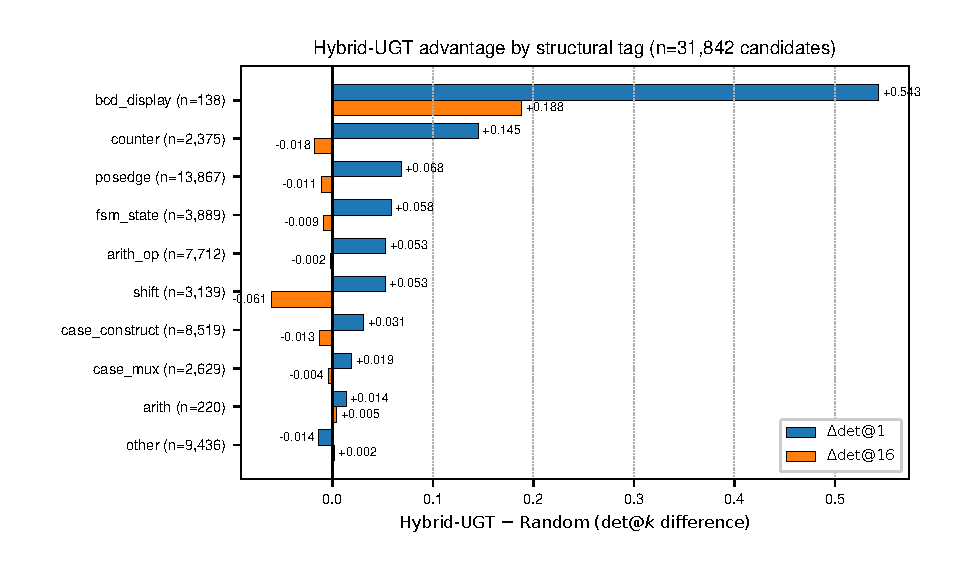
\includegraphics[width=\linewidth]{verilog_hybrid_struct_bar.eps}
\caption{構文タグ別Hybrid-UGT対Randomの差分（全件評価，31,842候補）．横軸はHybrid-UGTからRandomを引いた値．濃色のバーが$\Delta$det@1，薄色がdet@16．counter，arith\_op，posedge，FSM stateなどの主要タグで$\Delta$det@1が明確に正方向，shift/rotateで$\Delta$det@16が最大の負方向を示す．}
\label{fig:hybrid_struct_bar}
\end{figure}

\begin{figure}[t]
\centering
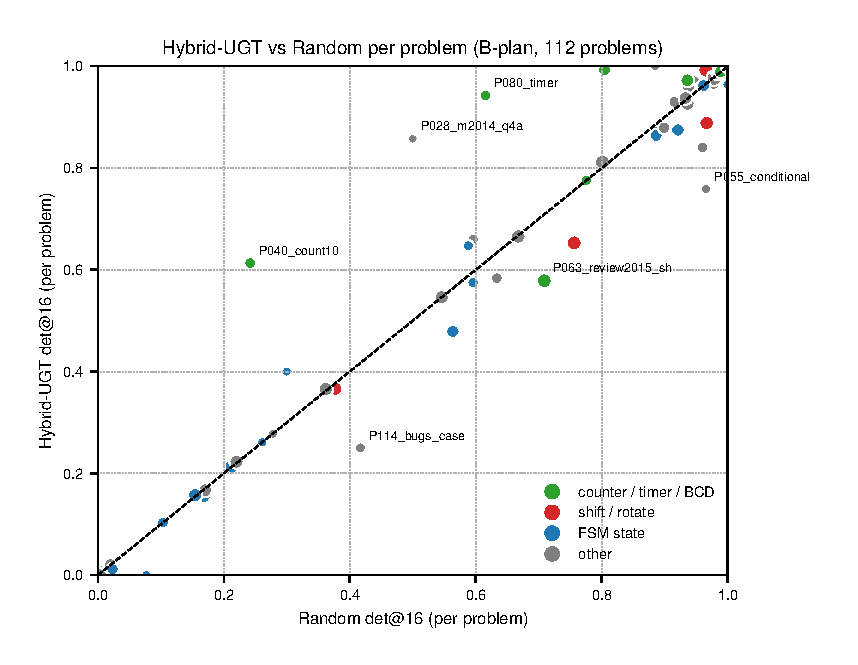
\includegraphics[width=\linewidth]{verilog_hybrid_per_problem.eps}
\caption{問題別Hybrid-UGTとRandomのdet@16散布図（全件評価，126問）．点の大きさは候補数（log scale）．対角線より上の点はHybrid-UGTがRandomを上回る問題．det@16では均衡，det@1では多くの問題でHybrid-UGTが上振れする．}
\label{fig:hybrid_per_problem}
\end{figure}

表\ref{tab:ugt_struct_full}と図\ref{fig:hybrid_struct_bar}に，候補が含むコード構造で問題群を分類した上でのHybrid-UGT対Randomの比較を示す．各候補は複数の構造タグに属し得るため，候補数は重複を含む．候補単位paired bootstrap (5,000-10,000 resamples) でゼロを跨がない有意な$\Delta$det@1がほぼ全主要タグで観測された：

\begin{itemize}
\item counter系（n=2,375）: $+0.146$ det@1 (95\% CI $[+0.126, +0.166]$)
\item posedge clock系（n=13,867）: $+0.069$ det@1 (95\% CI $[+0.062, +0.076]$)
\item FSM/state遷移系（n=3,889）: $+0.059$ det@1 (95\% CI $[+0.044, +0.073]$)
\item arith\_op系（n=7,712）: $+0.055$ det@1 (95\% CI $[+0.044, +0.067]$)
\item shift/rotate系（n=3,139）: $+0.053$ det@1 (95\% CI $[+0.039, +0.067]$)
\item case文（n=8,519）: $+0.032$ det@1 (95\% CI $[+0.021, +0.043]$)
\item case/mux（n=2,629）: $+0.022$ det@1 (95\% CI $[+0.002, +0.040]$)
\end{itemize}

「other」タグ（n=9,436）のみ$-0.014$と負方向だが，これらの問題は両手法ともdet@16$\geq 0.98$と容易な失敗が大半で，det@1の差は両手法のvector順序の偶然に大きく依存する．

一方，det@16では$\Delta$は全タグで$|\Delta| \le 0.018$と小幅で，唯一shift/rotate系（n=3,139）が$-0.061$ det@16 (95\% CI $[-0.078, -0.044]$) と顕著な負方向を示す．Counter系も$+0.146$ det@1から$-0.018$ det@16 (95\% CI $[-0.034, -0.002]$) に逆転する．これは「Hybrid-UGTのfocused vectorで早期にfailを露呈する候補は同じ；残るfailは$B$が大きくなるとRandomの広域サンプリングが偶然に踏むため，最終的な累積検出率がほぼ等しくなる」構造を示す．

Counter系での$+0.146$ det@1は，本稿のHybrid-UGTがdriveable inputが\texttt{reset}1bitのみの問題でも，smoke window内に\texttt{reset=0}を確実に含めることで，参照実装のカウンタ動作を早期に開始させて誤動作（例えば\texttt{count1to10}のoff-by-oneロールオーバー）を1サイクル目から露呈できることに対応する．Randomは50\%の確率でsmoke先頭が\texttt{reset=1}となりカウンタ起動が遅延するためdet@1が下がる．

\subsection{Span抽出からdirected inputへの変換}\label{sec:span_to_input}

Hybrid-UGT/Span-UGTは候補全体のスコアを並べ替えるのではなく，低確信度spanを具体的なvalidation input vectorへ機械的に変換する．例えばenable付きラッチ問題（\texttt{Prob028\_m2014\_q4a}）に対して，本稿の実装が行う処理は以下のとおりである．

\begin{enumerate}
\item 候補コード中の\texttt{if (ena)}分岐と\texttt{else}側代入の周辺が，bottom-16の低確信度トークン周辺spanとして抽出される．
\item span内のidentifierとinterface入力名の積集合から，焦点入力として\texttt{d}と\texttt{ena}を抽出する．
\item Span-UGTは焦点入力のみを動かすvector 2個を先頭に，続いてpart-select boundary・one-hot・alternating bit列・arithmetic boundaryを順に挿入する．Hybrid-UGTは先頭4個をrandom smokeに差し替える．
\item 同一signal-value tupleのvectorは重複除去する．順序回路ではseq\_fill\_cycles=8の保持期間で状態遷移を観察する．
\end{enumerate}

この変換は決定的（同じ$\text{SHA-256}(\text{problem},\text{trial},\text{candidate},\text{method})$からは同じ系列）であり，モデルや評価器の状態に依存しない．ただし§\ref{sec:problem_dependence}で示した通り，変換結果のdirected inputがRandom uniformを上回るタグは本実装では確認できなかった．Span抽出を強化して焦点信号を「直接駆動できる入力」だけでなく「内部信号を間接的に動かす入力」にも広げる発展が必要である．

\section{考察}

\subsection{candidate ranking分析の位置づけ}

Mean，Tail，MinLogPによるcandidate rankingは，本稿の提案手法ではなく，token log確率を候補全体の正誤判定に使うことの限界を確認する前提分析である．結果は，集約スコアがコンパイル失敗候補の後回しには有効である一方，コンパイル通過後のbit幅，状態遷移，境界条件，仕様解釈の誤りを十分に識別できないことを示した．Hybrid-UGTはこの結果を踏まえ，log確率を候補全体のスコアではなく，directed inputを作るための局所的なvalidation focusとして用いる．

\subsection{Hybrid-UGTのfail-fast優位性}

Hybrid-UGTがdet@1で全主要タグでRandomを上回る一方，det@16ではほぼ等値に収束するという性能曲線は，Hybrid-UGTの本質的な強みを表す．Hybrid-UGTは「smoke window内で明らかな失敗を踏みやすい入力」を決定的に置くため，多くのfailは1〜4ベクトル目で露呈する．Random uniformは確率的サンプリングのため，同じfailを踏むのに平均的に2〜4倍のベクトルを要する．

\subsection{Random baselineの強さ（高budget領域）}

一方，detection budgetが大きい領域（det@8，det@16）では，Randomは「Hybrid-UGTが見落とした失敗」を広域サンプリングで補い，両手法はほぼ等値に近づく．これは「Randomのcumulativeなsampling多様性が，後半でHybridのfocused inputの探索範囲を超える」ためと解釈できる．特にshift/rotate系では，shift量・回転量を全ビット幅にわたって試すRandom uniformの広域サンプリングが，Hybrid-UGTのpart-select boundary中心の入力よりも多くの誤動作を露呈する．

\subsection{Smokeでのreset制御の意義}

本実装のHybrid-UGTでは，interfaceにreset信号がある場合，smoke vectorの先頭2個が必ず\texttt{reset=0}と\texttt{reset=1}を両方含むよう強制する．Random uniformでは1bitのreset信号が50\%確率で初手\texttt{reset=1}になり，counter系のロールオーバー誤動作を1ベクトル目で踏めないケースが多い．Hybrid-UGTはspan内に\texttt{reset}キーワードが現れる候補を多く扱う性質上，「reset制御を意図的に行う」のは自然な延長であり，これがcounter系$+0.145$ det@1の主因である．

\subsection{Verilog専用手法としての位置づけ}

Hybrid-UGTはVerilogに特化した手法である．Verilogでは，信号名，bit幅，part-select，\texttt{case}，clock/resetがコード上に明示されるため，低確信度spanからinput stimulusを作りやすい．本稿では，この変換が明確なVerilog code-completionに対象を限定し，HDL検証における小規模validation input生成として手法を定義する．問題依存性の知見を踏まえると，Hybrid-UGTは「全Verilog候補を対象とする万能手法」ではなく，「特定の構文構造を含む候補について追加validation inputを設計する道具」として位置付けるのが妥当である．


\section{本研究の制約}

第一に，Hybrid-UGTはfailure detection手法であり，正しさを証明する手法ではない．生成validation input vectorで不一致が出た候補は失敗と判定できるが，不一致が出ない候補が正しいとは限らない．したがって，実運用では公式testbench，商用シミュレータ，形式検証，合成後検証などのfull validationが依然として必要である．

第二に，UGT評価は，正式生成済み候補のうちcompile-pass official-fail候補を抽出したオフライン評価である．この設定はfailure detection能力を分離して測るためには有用だが，候補集合全体に対する最終成功率や開発時間削減を直接示すものではない．評価対象は，全CPOF 34,805件のうち生成token数$\le512$の31,842件（91.5\%）であり，残り3,059件（8.5\%）はprompt logprobs再スコアリングのメモリ制約から除外している．特に長い候補ではHybrid-UGTの効果が変わる可能性がある．

第三に，本稿ではVerilogEvalの参照実装を用いて生成validation input vectorの出力比較を行った．実際の開発では常に参照実装が存在するとは限らない．その場合は，仕様assertion，既存golden model，プロパティチェック，または高信頼なsimulation modelをoracleとして使う必要がある．

第四に，主評価はQwen3.5-9B-AWQ-4bit，temperature=0.8，$k=10$に固定している．モデル，量子化方式，デコーディング設定が変われば，token log確率の分布や低確信度spanの意味も変わり得る．また，prompt logprobsを再スコアリングで取得する場合，追加の推論コストとメモリコストが発生する．

第五に，本稿のRandomベースラインはbit幅に応じた一様サンプリングである．これは産業的Verilog検証で広く用いられるconstrained random verification (CRV) や開発者がhand-craftするdirected testbenchを代替しない．本稿のHybrid-UGT評価は「uniform randomとの比較における機構的検出効率」を測ったものであり，CRVベースとの定量比較やHybrid-UGTのCRVへの統合は今後の課題である．特に，counter系$+0.145$ det@1やshift系$-0.061$ det@16といった効果量は本稿の評価設定における値であり，CRVが対象とするより構造化された入力分布の下での挙動は別途検証を要する．

第六に，本稿の評価結果は，本稿でgit管理下に再実装したパイプライン（span抽出，5手法のベクトル生成器，テストベンチテンプレート，iverilog/vvpドライバ）に依存する．低log確率tokenからspanを切り出して焦点信号や境界値を抽出するロジック，および順序回路における各vector後のfill cycle数（本稿では8サイクル）といった実装詳細は，過去文献の記述だけからは一意に確定しない．従ってtag別の効果量は実装が異なれば変化し得る．本稿は，論文の主張を「specific aggregate detection rate」ではなく「論文中の手法仕様に基づく再現可能なreference implementationにおける挙動」として位置付ける．

\section{結論}

本稿では，LLMによるVerilogコード生成候補に対し，token log確率を用いた不確実性誘導テストを提案・実装・評価した．まず，VerilogEval 156問・156,000候補を用いてMean，Tail，MinLogPによるcandidate rankingを評価し，log確率集約スコアはコンパイル失敗候補の後回しには有効だが，コンパイル通過後のsemantic correctness識別には限定的であることを示した．

この限界を踏まえ，低log確率tokenの位置を局所的不確実性spanとして扱い，span内の信号名，bit範囲，演算子，case/state，reset/clockから小規模directed validation inputを生成するHybrid-UGTを提案した．本稿では，サブサンプリング選定，prompt logprobs再スコアリング，span特徴抽出，5手法のベクトル生成器，testbench生成，シミュレータドライバ，並列orchestratorからなる評価パイプライン全体をgit管理下で再実装した．

compile-pass official-fail候補のうち生成token数$\le 512$の全件31,842候補に対する評価では，Hybrid-UGTがdetection budgetの小さい領域でRandomを明確に上回ることが示された．全体でdet@1は0.524（Random 0.496，$\Delta=+0.028$），counter系（n=2,375）で$+0.145$ det@1，posedge clock系（n=13,867）で$+0.068$ det@1，FSM/state遷移系（n=3,889）で$+0.058$ det@1の優位を示した．一方，det@16ではHybrid-UGT 0.841，Random 0.845と同等に収束し（$\Delta=-0.004$），shift/rotate系（n=3,139）でのみ$-0.061$ det@16の顕著な劣後が残る．

この性能曲線は，Hybrid-UGTを「少数validation vectorで明らかなfail候補をfail-fast棄却する」per-request screeningの用途に位置付けることを支持する．Random uniformは$B$を増やせば最終的に同等の累積検出率に達するが，1〜4ベクトル目で多くの失敗を踏み落とすHybrid-UGTの方が，screeningコスト最小化の観点では有利である．今後は，(i) span抽出ロジックの強化（output駆動の挙動や状態変数を間接的に動かす入力の自動推定）によるshift/rotate系のdet@16改善，(ii) constrained random verificationとの統合・比較，(iii) より多くのVerilog構造（テストベンチ依存の入力タイミング，async reset，clock-domain crossing）への手法拡張，(iv) 別モデル・別ベンチマーク（VerilogEval-Specification，RTL-Coder）での汎化性検証，が必要である．

\bibliographystyle{ipsjunsrt}
\bibliography{references}

\end{document}
